% \graphicspath{{tex/figs/ch2}}

\chapter{Background: Expressive Performance}\label{ch:ch2}
This project is based upon two major research components. The first is the MIR problem domain of expressive musical performance, and the second is the modeling domain of Transformers. In this chapter, we will introduce and discuss EMP. In chapter \ref{ch:ch3} we'll do the same for the Transformer. 

Expressive musical performance is a small subset of Music Information Retrieval research, which we broadly categorized into two separate tasks: the first is developing computational methods for musical analysis, the second is developing computational methods for music generation. We are interested in generative models, although it is worthwhile to note that there is considerable overlap between the two areas\footnote{Creating a performance generation system is useful for performance analysis as long as the generation system is interpretable. The reverse is also true. Analysis provides insight to generation, and generation provides insight to analysis}. A proper knowledge of the entire musical generation process as a whole is necessary to understand how EMP generation models work. \citet{ji2020comprehensive} break the generation process into three stages with four different roles that interact with that process at each stage. Figure \ref{fig:generation_process} shows each step in the process as well as the agents that participate\footnote{This figure is our reproduction of a similar image presented by \citet{ji2020comprehensive}}. 

\begin{figure}
    \centering
    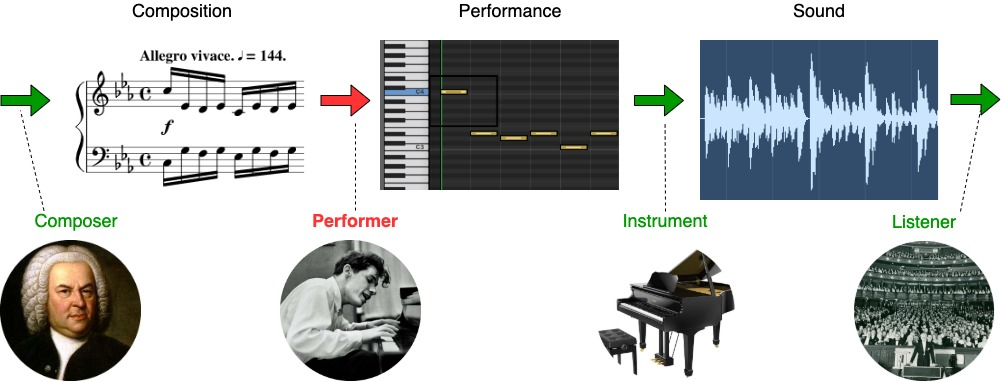
\includegraphics[width=1\linewidth]{figs/ch2/musical_generation.jpg}
    % \missingfigure{Image that shows different components of musical generation process}
    \caption{The first step of musical generation is composition, shown as a score in the figure. The second is performance, our area of interest, and is indicated by a MIDI file's piano roll representation. The third is the production of sound, shown as a raw audio wave. Each different agent: composer, performer, instrument, and listener, can be thought of as a separate computational model in the generation process}
    \label{fig:generation_process}
\end{figure}

An EMP generation model is analogous to the performer shown in \ref{fig:generation_process}, who takes as input a composition and produces as output a performance. We define musical expression as the performers' interpretation of a composition codified into different performance parameters intended to contribute to the quality of a musical experience% 
\footnote{As has already been mentioned and as will show in detail later in this work, defining the ``quality'' of musical experience is no minor task. Such a definition is necessary to train performers (either computer or human) to create desirable performance.}. 

Figure \ref{fig:generation_process} shows that a performer interacts with a composed score to create a performance. To more clearly define EMP generation, we start by describing the essential elements of both scores and performances. This chapter's descriptions are not intended to be at a detailed mathematical level but the general musicological level. We provide feature definitions, which contain the score and performance information embedded at a mathematical level and are necessary for building any computational model, of some of the EMP models upon which our work is based in section \ref{sec:emp_generation_models}. We refer the reader to appendix \ref{ase:app_one_sect_1} which provides some basic musical terminology and concepts that will be useful for understanding our definitions\footnote{Most of the appendix material may seem elementary to those who already have a background in music or musical notation}. Due to the constraint of our data, we focus only on western classical piano music. 

\section{Scores}\label{sec:scores}
Scores are symbolic representations of a musical composition. They are expressed through a language of symbolic notation used to express musical ideas and information. Scores present this information in a hierarchical structure with different levels of musical detail at each level. Figure \ref{fig:score_hierarchy} shows a sample score and the different hierarchical levels of information that it contains

\begin{figure}
    \centering
    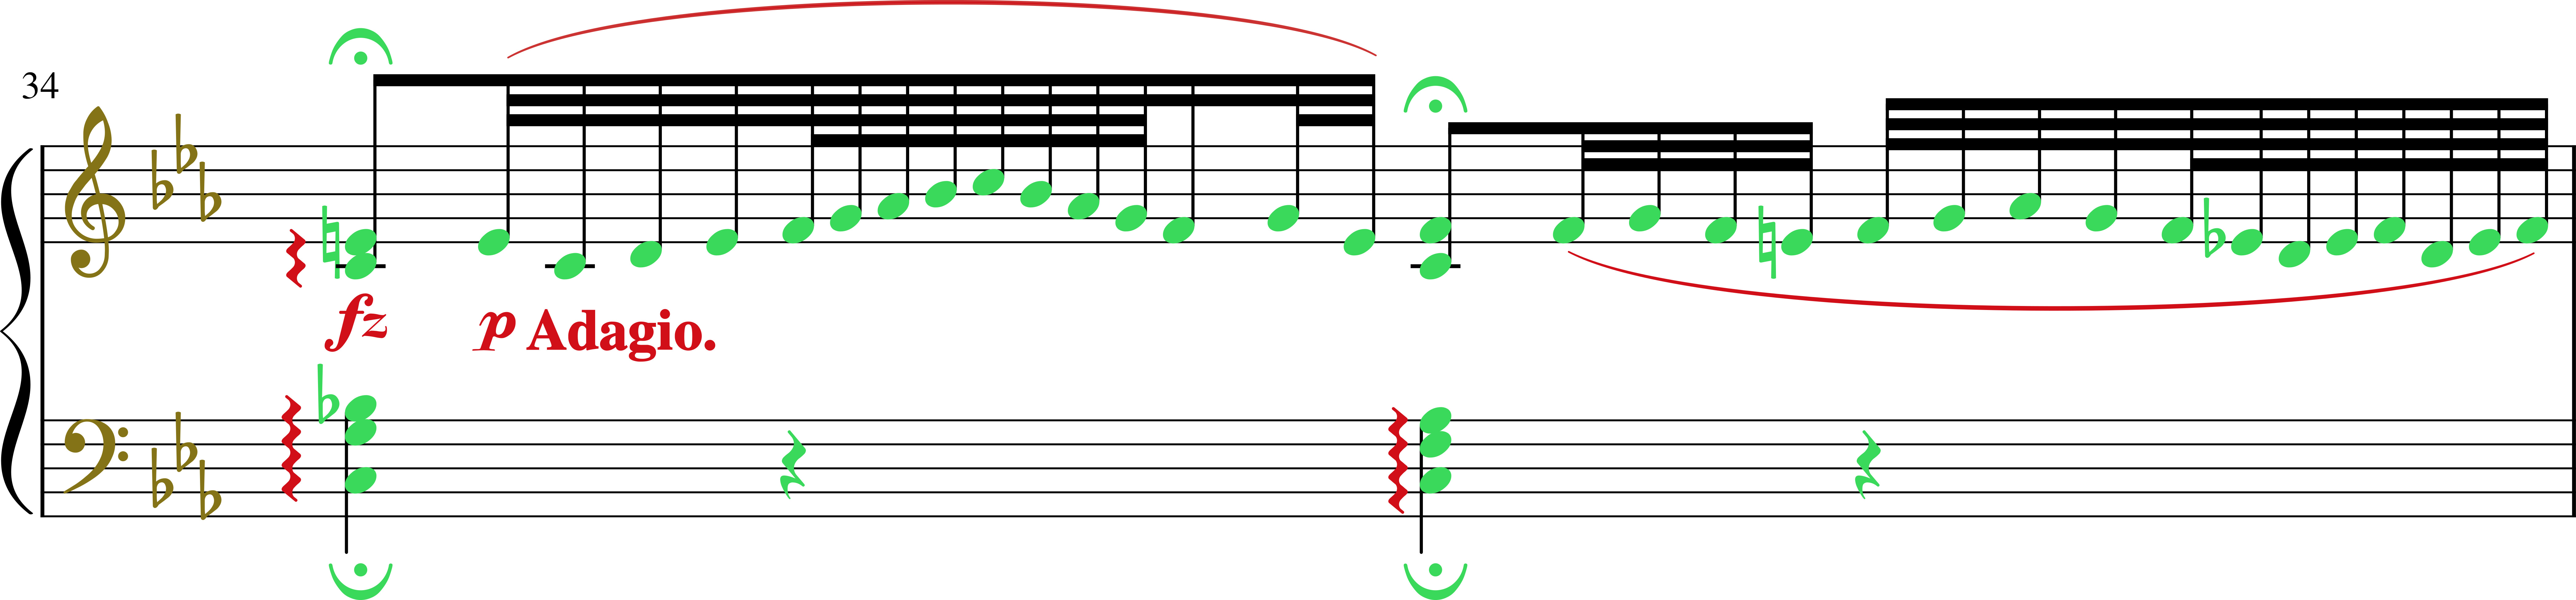
\includegraphics[width=1\linewidth]{figs/ch2/score_hierarchy.jpg}
    % \missingfigure{Image that shows a sample score with colorized annotations that show the different hierarchical levels}
    \caption{A sample hierarchy of a score delineated by different colors. The green shows the low level, which includes the pitch and timing of every note. The red represents the mid-level which shows dynamics and tempo information about local musical substructures. The tan color illustrates the high level, and includes the key and time signatures.}
    \label{fig:score_hierarchy}
\end{figure}

%mnot for musical notation. Bold and emphasize at once
\newcommand{\mnot}[1]{\textbf{\emph{#1}}}

The lowest level contains information about the pitch and timing of every single note, as well as optional information about how the note should be played. This can include information specific to instruments such as the bow direction of a violin, but for our purposes (dealing only with piano) we will consider this to be the articulation of each note, usually indicated by \mnot{legato} or \mnot{staccato} \rtodo[,inline]{Make sure to have some background information on articulation in the appendix}

The middle level contains information related to certain substructures within the musical composition, which are usually expressed within a grouping of notes or measures. The most common score annotations at this level are dynamic markings which indicate whether to play a grouping of notes as \mnot{f} (loud), \mnot{p} (soft), or as a \mnot{crescendo} or \mnot{decrescendo} (gradually increase or decrease the volume). %\rtodo{Add correct notation markings) %
Although dynamic markings are the most common at this level, it is also possible to see score markings for all other musical features, such as local tempo or articulation of a certain substructure. Perhaps the most important score marking at this level is that of a phrase, which is a marking that indicates that a group of notes should be interpreted as belonging to a singular musical idea and that each note should fit within the context of the phrase as a whole. A phrase can be expressed through all of the different aforementioned musical features, including the tempo, timing, dynamics, and articulation of the notes.

The highest level contains meta-information that relates to the entire composition as a whole. This information typically includes the key signature and time signature, as well as the global tempo for the entire piece, most commonly represented as BPM. 

% \subsection{Score Features}
% \rtodo[,inline]{This entire section needs work. Include some detailed information but refer reader to chacon's thesis for a full breakdown. Possibly mention features from virtusoNet}.

% There are some score features which are required for EMP models, which include the musical features at the lowest level of a score as explained in section \ref{sec:scores}. These are pitch and timing, and the duration of the notes. Mid-level features include concepts at the local level and have some music theoretic concepts, such as downbeat information of a given measure according to the time signature, or the tonality of a chord (tonic, dominant, etc). High-level features represent advanced music theoritic concepts that are more global to the entire piece, including abstract properties of the piece such as the emotion the piece should convey and how different sections of the piece relate to each to tell a complete story \cite{eduardo2018computational}. 

% Both the mid-level and high-level features are not necessarily required for every EMP model as the lower-level features are, and are not consistent across all EMP models. It still remains an open question as to which features should be extracted from the data that the model can learn from. The lack of consistency in these features is one of the reasons that evaluation of EMP generation models is so difficult, as explained in section \ref{sec:evaluation}. 


\section{Peformance}\label{sec:performance}
An expressive musical performance contains most of the same musical information as does a score, including pitch, tempo, timing, and articulation. However, there is one key difference between the two. Expressive performances will deviate (or interpret) from the exact information given in the score. For example, although a score may indicate a tempo of 120 BPM, it is unlikely that a given performer will perfectly adhere to this tempo throughout the piece's entirety. This interpretation is even more apparent if the score indicates a change in tempo somewhere in the composition. If a score contains an \mnot{accelerando}, meaning that the performance should speed up over a series of notes, there is no precise indication of the rate at which the tempo should increase. Some performers may choose to speed up at a fast pace and over a short period. Others may decide to increase the tempo at a slow rate and over a more extended time period. A single \mnot{accelerando} can ``correctly'' result in either of these outcomes. 

Each expressive parameter will be measurable and absolute, whereas the score markings of these features are more of a suggestion than a rule. Performance has a few additional components that are not necessarily indicated in scores but are relevant in the context of performance alone. The first we will refer to as deviation, which is heavily related to timing. It is represented as a numerical number that represents how far off the timing of a particular note deviates from its ``correct'' position in the score. These micro-timing deviations present in musical performances are an essential part of expression. Without them, each note onset and offset would fall precisely in line with its marking in the score. This is how current commercial EMP generation systems operate, resulting in performances that are deterministic, robotic, and mundane \rtodo[,inline]{add a reference, graphic, and sample performance}. 

Pedaling in piano performance is another important feature of performance that is not always present in a score. There are several different types of piano pedals. The most common are the sustain pedal, which prolongs every notes' duration when activated, and the soft pedal, which softens the entire piano's sound. Although these pedals' effects are directly related to the articulation and dynamics of the performance, their presence (or lack of) is a crucial component of piano performance. The sustain pedal is actively used in almost all modern piano performance, even in the absence of pedal score markings. 

% \subsection{Performance Features}
% \rtodo[,inline]{Similarly to score features section, provide more detailed information about some of the math behind the features. Cite other resources where necessary}
% For western classical solo piano music, performance features are relatively simple compared to the score features as well as to other instruments. Most EMP models use the different aspects of a piano performance as explained in section \ref{sec:performance} for their data features, including the pitch, tempo, timing (or timing deviation), articulation, and pedal. Although at an abstract level the features are the same, there are different numerical methods used to describe each of the different aspects. These are presented in \rtodo[,inline]{Add reference to relevant work section that goes over the different elements. This information may belong better here and then referenced in the relevant work section}. 

\section{Data}
The data required for EMP generation includes a digital representation of a score and a corresponding performance. MusicXML, a text-based representation of a composition, is the most common data format for a score. Performances could directly be represented through raw audio, which is widely available on the internet. Instead of audio however, an intermediate data form, MIDI, is commonly used to constitute the performance. MIDI is an event-based data format and software interface that contains information about different aspects of a recorded performance. This information includes the recorded timing, pitch, and volume of every note, the instrument used, and pedal information (specifically in the case of piano performance). 

There are several reasons for the preference of MIDI over raw audio. The first is that audio data is inherently noisy, sparse, and larger in its dimensionality and size. Using audio to represent performance requires a significant compression of natural frequencies into more abstract musical representations such as pitch -- MIDI natively contains these abstractions. MIDI also better aligns with the generation process outlined in \ref{fig:generation_process} in which performance is seen separate from sound synthesis and allows computational models to define such boundaries easily. In the full generation process, a different model would be used to take the performance data in MIDI and synthesize it into raw audio presented to the listener. 

Both MIDI and MusicXML contain all of the required information to represent all of the musical components of both a score and a performance, including pitch, tempo, timing, articulation, deviation, and pedal. See appendix \ref{ase:app_one_sect_2} for more information on both MusicXML and MIDI. 

Computational models that deal with the relationship between scores and performances often need additional metadata about the alignment between every note in both the score and performance. This metadata is generated by running a performance and its corresponding score through a data alignment process in which every performance is matched to a marking in the score. Given the highly dynamic nature of musical performance, it is a non-trivial task to run this alignment process for a set of scores and performances, especially if the task is performed by manual human annotation. There exist methods for both manual and automatic alignment. Due to the time-consuming nature of manual alignment and the need for large data sets to build higher quality models, automatic alignment algorithms are an active area of research.

\begin{figure}
    \centering
    \missingfigure{Show why score to performance alignment matching is necessary.}
    \caption{Two performances of the same score can vary wildly in their tempo and timing. This makes it necessary to have a score to performance alignment for every performance. }
    \label{fig:alignemnt}
\end{figure}

\subsection{Existing Data Sets}
\rtodo[,inline]{Rework this section to fit with new paper outline. Need to forward reference models instead of back reference}
One of the problems facing EMP and MIR is the lack of high-quality and large-scale datasets\cite{cancino2018computational}. The broad scope and diversity of data across the different musical components partly explain this absence. As has been discussed, there are different stages in the musical process, and there are different ways to represent music at each stage. For example, composition can contain the same amount of information in at least three forms. The first and most common is the symbolic representation in the form of a data format like MusicXML. As we have seen, we can infer much of the information necessary to construct a score from performance alone, given that performance contains the timing and pitch of every note. Such score information is naturally embedded in both MIDI and raw audio. 

The biggest hindrance in data gathering is that most of the musical data available on the internet is in the form of audio. As we have pointed out, processing audio data for musically plausible purposes is difficult compared to other better-suited formats. While a fair amount of MusicXML and MIDI does exist, it is relatively small compared to the amount of audio data. We draw a comparison to the data used in NLP research, where textual data is analogous to MusicXML and MIDI, and speech audio is analogous to musical audio. One of the reasons NLP has been able to significantly advance its progress in the last few decades is because of the massive amount of readily available textual data on the internet. If NLP only had available text data as represented by audio, as is often the case with music, it would be significantly more challenging to develop NLP systems and applications. Nevertheless, there has been a recent effort to gather quality data in MIR. We present some of these datasets as they are relevant to EMP. 

There are normally 3 required components for a EMP dataset. 
\begin{enumerate}
    \item Scores (usually in the form of MusicXML)
    \item Performances (usually in the form of MIDI)
    \item Metadata about the matching alignment between the score and performance. 
\end{enumerate}
Score data can be gathered by finding readily available MusicXML files from open source software projects which contain music that is in the public domain (which all western classical music is) \footnote{\href{https://musescore.com}{MuseScore} is the most common. Also see the \href{https://imslp.org/wiki/Main_Page}{International Music Score Library Project}}, or by using Optical Music Recognition (OMR) to automatically scan paper sheet music into a digital form followed by manual corrections where needed. MIDI performances can only be recorded when a performer uses an instrument that is compatible with the MIDI protocol. Although there are many digital piano keyboards with this combability, semi-professional and professional pianists primarily play on acoustic pianos. Some computer-controlled acoustic pianos can record MIDI performance, such as the Yamaha Disklavier and the older Bosendorfer CEUS system. Therefore, MIDI data of professional piano performance has historically been limited to performances on these piano systems. 

There is no standardized method for score-to-performance alignment methods and data representations. Each dataset presents its own alignment method as well as the metadata that represents the alignment. 

To provide context for the progression of data used in EMP generation, we will introduce an older dataset used in EMP research, the Magaloff Corpus. We then describe a much larger scale dataset, the Piano-e-competition, which has recently been adapted for EMP generation use.~\citet{cancino2018computational} give a full overview of datasets used in EMP generation. 

\subsubsection{Magaloff Corpus}
Nikita Magaloff was a Russian pianist known for his performance cycles of Chopin's entire works for the solo piano. In one of his final cycles of performances recorded in 1989, he played on a Bosendorfer SE computer-controlled piano.~\citet{flossmann2010magaloff} obtained special permission to access the MIDI data from this performance cycle. They gathered score data using OMR with manual corrections where needed.  The alignment method of~\citet{grachten2006expressivity} was used to produce the note-matching annotations, along with manual corrections. The dataset contains over 10 hours of playing, 150 compositions, and over 320,000 performed notes. The corpus, however, is not publicly available and has only been used in research by \citet{flossmann2010magaloff} and colleagues \cite{eduardo2018computational}. 

\subsubsection{Piano-e-competition}
As has been discussed, there is a large push in modern MIR to produce high-quality large datasets. At the heart of this research in MIR is the Piano-e-competition. Started in 2002, it is an international piano competition which attracts some of the promising up and coming musicians at both the senior and junior level \cite{the-disklavier-education-network}. Every performance from the competition is played on a Yamaha Disklavier and is recorded in both MIDI and audio. Due to the data set's size and availability, it is commonly used in MIR research. There exist several different adaptations of the original data that are specific to particular research purposes. 

The first of these is the MAESTRO (Midi and Audio Edited for Synchronous TRacks and Organization) dataset. \citet{hawthorne2018enabling} introduce the MAESTRO dataset, which presents both MIDI and audio data from the Piano-e-competition in a canonical and easily accessible form. The dataset was first used to build a full musical analysis and generation process framework named wav2midi2wave. This framework includes a musical transcription process \cite{hawthorne2017onsets} from raw audio to midi (wav2midi), a direct musical composition and performance generation model \cite{huang2018music} \footnote{This model directly generates MIDI files without using scores. It simultaneously generates a composition and performance. This direct generation is a merging of the two separate tasks into one as shown in figure \ref{fig:generation_process}} (can be seen as the midi or midi2midi part of the wav2midi2wav framework), and a synthesis model that takes MIDI and generates raw audio\cite{oord2016wavenet} (midi2wav). The MAESTRO dataset is the most commonly used form of the Piano-e-competition data. 

The Piano-e-competition also forms the basis for a data collection, which we will refer to as the KAIST dataset\footnote{We take the name from the KAIST Graduate School of Technology, which the researchers who created the dataset work for}. The Piano-e-competition dataset itself does not provide any score data about any of the compositions used in performance. The KAIST dataset was created specifically for an EMP generation system, and therefore needs score data for every performance recorded in MIDI. This score data was collected by \citet{jeong2019virtuosonet} by downloading MusicXML files online, mostly from MuseScore. On top of gathering the score data for all performances in the Piano-e-competition, \citet{jeong2019virtuosonet} also run the automatic score-to-performance alignment algorithm of \citet{nakamura2017performance} to provide metadata about the alignment between each score and performance. Automatic score-to-performance alignment is error-prone, especially in the case of performance mistakes\footnote{A mistake in the performance results in a performance note having no correct match with a score note.} As a result, some performance notes are not aligned to those in a score. Due to the possibility for error in automatic alignment, \citet{jeong2019virtuosonet} also add additional manual and heuristic corrections to the alignment where needed. 

Other than the discrepancy in scale, the most significant difference between the KAIST dataset and the Magaloff corpus is that the KAIST dataset contains multiple performances for the same score. In contrast, the Magaloff Corpus has a 1-1 mapping between a score and performance. The KAIST dataset has 226 scores across 16 different composers, roughly 660,000 score notes, and around 3,500,000 performance notes. The number of matched performance notes is ten times larger than the Magaloff Corpus, and all data is publicly available \footnote{The dataset is open sourced at \url{https://github.com/mac-marg-pianist/chopin_cleaned}}. 

The Aligned Scores and Performances (ASAP) dataset~\cite{foscarin2020asap} is a recent adaptation of both the KAIST dataset and the MAESTRO dataset. It uses the MusicXML files from the KAIST dataset, audio from the MAESTRO dataset, and MIDI files from both sources extracted from the common origin of the Piano-e-competition. It provides additional alignment metadata for both MIDI and audio and more manual correction in the MusicXML score files. Although the purpose of the ASAP dataset is for Automatic Music Transcription (AMT)\footnote{AMT is the task of transcribing a score from a performance (either in audio or MIDI form). AMT is the "opposite" of EMP. It maps a performance to a score instead of a score to performance}, it is just as equally useful for EMP generation. To our knowledge, it hasn't seen an application in any EMP generation task. Although it is mostly similar to the KAIST dataset, the implications of its extensions are undetermined in EMP research. 


\section{Performance Evaluation}\label{sec:evaluation}
Evaluation is an essential component of developing ML models. A models' evaluation is a measure of its quality and serves as a benchmark that can be compared to other models in the same domain. Due to the inherently subjective nature of music and musical performance discussed in chapter \ref{ch:ch1}, evaluation is notoriously difficult to understand and define correctly for EMP generation models~\cite{cancino2018computational}. 

The evaluation of computational models, specifically for EMP models, is typically categorized in two ways: quantitative and qualitative evaluation. Quantitative evaluation methods involve using numerical metrics, which are computationally generated and deterministic. Qualitative evaluation methods usually involve human feedback and judgment, often presented in some standardized statistical measures. The key difference between quantitative and qualitative is that qualitative methods are not as consistent and more challenging to reproduce, given the reliance on human listeners' subjective feedback. Quantitative evaluation methods are traditionally preferred over qualitative because of their consistency and reliability. However, in the case of music generation models, qualitative evaluation methods may be more relevant because of music's highly subjective nature. Finding suitable methods of evaluation is an active area of research in EMP \cite{cancino2018computational}. 

\subsubsection{Quantitative Evaluation}
There are several different metrics commonly used in the evaluation process, all of which are specific to the type of data and problem domain the model fits inside. Our model is a regression model, which we cover in chapter \ref{ch:ch5}, and so we present some standard metrics used to evaluate regressive EMP models. 

The two common metrics used for evaluation and regression are Mean-Squared-Error (MSE) and the Coefficient of Determintation (commonly abbreiated as $R^2$). MSE is used to measure the difference between a prediction and an actual observed target value, and can be denoted as $MSE = \frac{1}{n}\sum_{i=1}^{n}(Y_i - \hat{Y_i})^2$, where $Y_i$ is the observed value at time step $i$, and $\hat{Y_1}$ is the predicted value. $R^2$ is a probablistic measure of the linear correlation between variables $X$ and $Y$, and is denoted as $\rho_{X,Y} = \frac{cov(X,Y)}{\sigma_{X}\sigma_{Y}}$ where cov indicates the covariance and $\sigma$ indicates the standard deviation.

\subsubsection{Qualitative}
Qualitative evaluation in EMP is most often conducted by presenting computationally generated performance to human listeners and gathering feedback and judgment. Although there have been efforts to standardize this evaluation process, the qualitative evaluation methods of different EMP models significantly vary. The lack of consistency in the evaluative methods makes reproducing experiment results difficult in EMP research, but it is still perhaps the best way to evaluate EMP models today. 

The most significant effort in EMP generation qualitative evaluation was the Performance Rendering Contest (Rencon)~\cite{katayose2012evaluating}. Starting in 2002 and ending sometime around 2013~\cite{cancino2018computational}, Rencon was an annually held competition that provided a way to compare EMP systems using standardized and evaluation methods. It did so by subjecting each models' performances to the same listening judges and judgment rubric, thus adding a higher level of confidence in each model's final quality judgment. 

Although the evaluation methods changed from year to year, they all followed the same general structure. To enter the competition, contestants would submit MIDI files of generated performances by their respective models. The choice for compositions was usually restricted to a small set of composers, such as Chopin or Mozart. A Yamaha Disklavier was then used to create an acoustic rendering of the generated MIDI file played in front of a set of judges. The judges' makeup usually included musical experts with varying experience. The judges submitted a feedback survey that would rate aspects of performance such as "rhythmic accuracy," "musical skill," and "overall quality," along some standard statistical scale. A winner was chosen according to the judge's survey entries. 

Although Rencon does not currently hold competitions, it forms the basis for many of the methods used in the qualitative evaluation of EMP models. As mentioned, the exact survey methodology and the judges' makeup varies across different experiments \cite{jeong2019virtuosonet, schubert2017algorithms}, but the general method is the same as that of the Rencon. This general consistency across methods is somewhat apparent when considering that these evaluation methods are mostly the same as those of contests that involve real human performers, such as the Piano-e-competition. 

There are some methods of qualitative evaluation which don't follow the listening test method of Rencon. They usually involve a mixture of both computational and human analysis. Such methods may use computation to generate visualizations or find patterns in performance data, which a researcher then interprets in a qualitative way~\cite{widmer2009yqx,jeong2019score, grachten2012linear}. There are also more informal listening-based evaluation methods, in which the feedback given by the listening judges exists not as a statistical measure but as general feedback and reaction~\cite{oore2020time}
